

\section{Implementation}
\label{section:implementation}

We extract aliases for entities from Wikipedia automatically both using API and using the actual page content, then apply pattern matching rules for slot value extraction. Our contribution is that we perform pattern matching that conforms to each slot value along with post-processings to eliminate noisy outputs. 

%\ceg{Instead of this paragraph we talk about what this %section will
%contain. We can discuss the input/output of the system %too.
%}

\subsection{Alias Generation}
\label{section:aliasgeneration}


\subsection{Cumulative Citation Recommendation}
\label{sec:ccrimpl}

Our pipeline of processing the corpus consists of a two layer indexing system referred to as \textit{Chunk Files Index Generator} and \textit{StreamItems Index Generator}. Chunk Files Index Generator will generate indexes of the chunk files that contain a mention of any of the desired entities. StreamItems Index Generator 
on the other hand will index StreamItems that contain a mention of a given entity respectively. This two level indexing will eliminate the need to process each and every ChunkFile/StreamItem for every entity. The reason for splitting this task into two steps is that not all chunk files contain any mention of the entities and 
we want to get rid of them as soon as possible. Chunk Files Index Generator which discards non-mentioning chunk files and will stop further processing a chunk file as soon as it finds a mention there. Each chunk file can contain up to thousands of SIs which can be so time consuming if we were to process them in our Java base code. Processing StreamItems on the other hand is done in Java with ideas in mind for later on extensibility by adding other Java libraries.



\subsection{Streaming Slot Value Extraction}
\label{sec:ssve}
\begin{figure}
\centering
%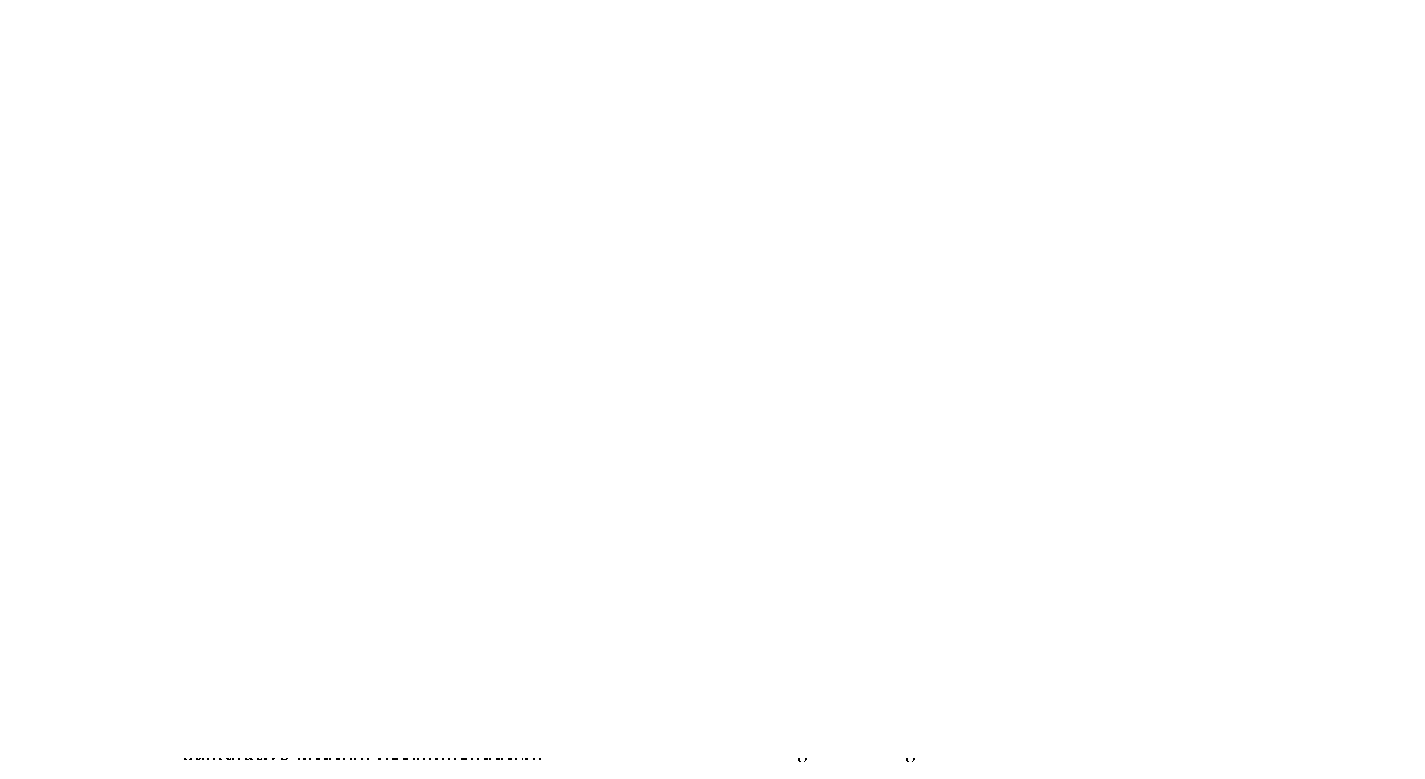
\includegraphics[width=4.5in]{./images/system.eps}
%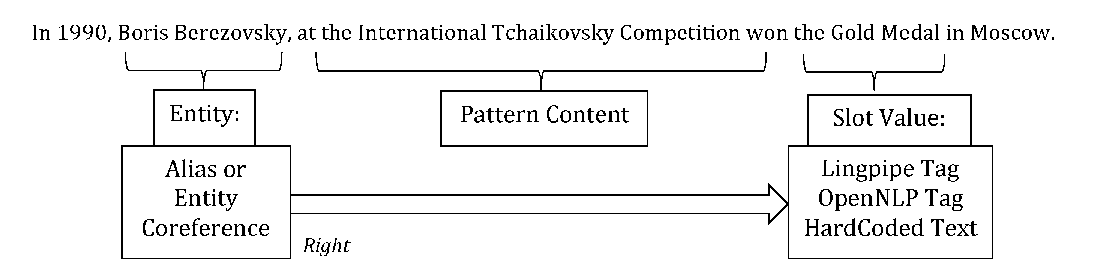
\includegraphics[width=6in]{./images/Pattern.eps}
%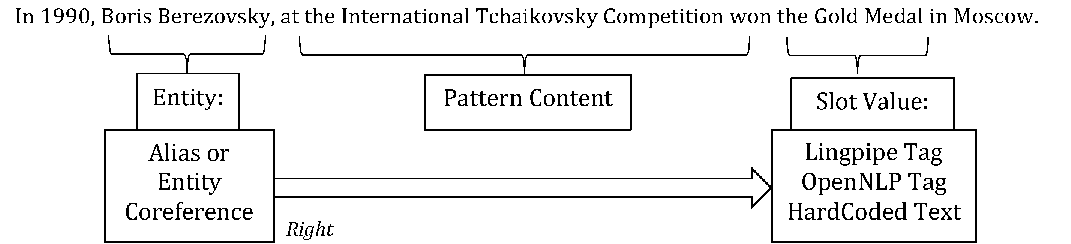
\includegraphics[width=6in]{./images/Pattern-eps-converted-to.pdf}
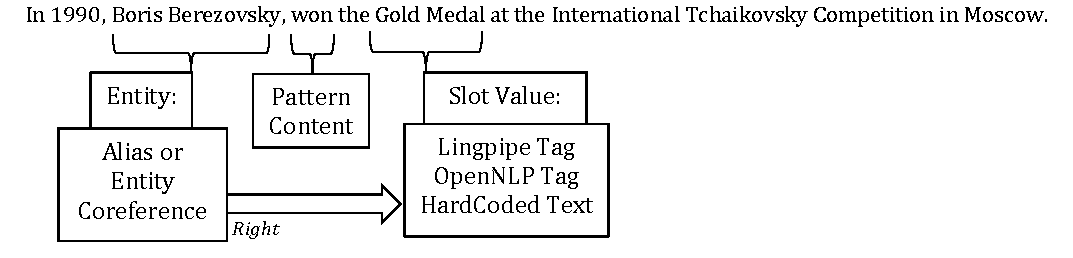
\includegraphics[width = 13cm]{./images/Pattern-crop.pdf}
% cropped pdf created using $ pdfcrop Pattern.pdf
\vspace*{-.1in} \caption{Pattern Matching with Slot Value on the Right Side of Entity. }\label{fig:pattern}
\vspace*{-.2in}
\end{figure}

In the data set, we are given a date range of documents as training data. Instead of building a classifier we use pattern matching methods to find corresponding slot values for entities. 
Pattern matching is simple to manipulate results and implement. Additionally, a classifier approach is more difficult to evaluate and explain results.

With the StreamItem indexes generated by the CCR, we first fetch the sentences containing entites by using alias names and coreference information provided by Lingpipe tags. Then use these senteces to match patterns and when patterns matched, generate SSF results.

\begin{algorithm}
  \caption{Streaming Slot Value Extraction Pseudocode}
  \textbf{List of entities $\mathcal{E} = \{e_0, \ldots, e_{170}\}$}\\
  \textbf{List of patterns $P = \{p_0, \ldots, p_{|P|}\}$}\\
  \textbf{List of streamitems containing entities $\mathcal{S} = \{s_0, \ldots, s_{|\mathcal{S}|}\}$}\\
  
  \begin{algorithmic}%[1]
    \FOR{$si \in \mathcal{S}$}
      \FOR{$sentence \in si$}
        \FOR{$entity \in \mathcal{E}$}
	  \IF{Contains($sentence$, $entity$)}
          %%\IF{check\_pattern(sentence, pattern)}
            \FOR{$pattern \in P $ suitable for $entity$} 
              \IF{Satisfies($sentence$, $pattern$)}
                \STATE Emit($sentence$, $pattern$)
              \ENDIF
	    \ENDFOR
          \ENDIF
        \ENDFOR
      \ENDFOR
    \ENDFOR
  \end{algorithmic}
\end{algorithm}


\subsubsection{Format of patterns}
A pattern is defined as a record representing knowledge going to be added to a knowledge base. A pattern $\mathcal{P}$ is represented as a five-tuple $\mathcal{P} = \langle p_1, p_2, p_3, p_4, p_5 \rangle$.


The first value, $p_1$ represents the type of entity. These entity types are in the set $\{ \text{\tt FAC}, \text{\tt ORG}, \text{\tt PER} \}$ where \texttt{FAC} represents a type of facility, \texttt{ORG} represents an organization and \texttt{PER} represents a person. \texttt{FAC}, \texttt{ORG} and \texttt{PER} are Lingpipe entity types. The $p_2$ represents a slot name. A list of slot names is present in Table~\ref{table:slotNameOntology}. The third element $p_3$ is the pattern content. This is a string found in the sentence. The extractor looks for this exact string or pattern in a sentence. The pattern evaluator uses a direction (\texttt{left} or \texttt{right}) found in $p_4$ to explore sentence. The final element $p_5$ represent the slot value of a pattern. This %When we match one pattern, we match all the 
%fields except the third field, which is extracted as the final result.
The type of slot value may be the entity type tagged by Lingpipe, a noun phrase (\texttt{NP}) tagged by OpenNLP or a hard-coded phrase. For these three kinds of patterns, we implement them in different 
ways accordingly. Next, we explain the patterns with more details, an example can be found in Figure~\ref{fig:pattern}. 



\subsubsection{Types of patterns}
There are three types of patterns distinguished by different types of slot values in the patterns. The matching methods using these three types of patterns are implememented according to the different information and structures of slot values.

 
\textbf{Type I.} This pattern type is driven by the slot value type, a pattern tagged by Lingpipe. For example, pattern $\langle$\texttt{PER, FounderOf, \textit{founder}, right, ORG}$\rangle$. \texttt{PER} means 
that the entity we are finding slot values for a PER entity; \texttt{FounderOf} means this is a pattern for FounderOf slot. \textit{founder} is the anchor word we are match in a sentence; \texttt{right} means that we are going to the right part of the sentence to match the pattern and find the slot value; ORG means the slot value should be a ORG entity.

\textbf{Type II.} This pattern type is unique because it only looks for a slot value tagged as noun phrase (NP) by OpenNLP.\@ For example, pattern $\langle$\texttt{PER, AwardsWon, \textit{awarded}, right, NP}$\rangle$. This pattern can be interpreted as that we are looking for a noun phrase after the \textit{awarded} since that noun phrase may represent an award. Titles and awards are usually not the Lingpipe entities, hence the use of the OpenNLP noun phrase chunker to fetch the noun phrases.

\textbf{Type III.} Some relations are best discovered by hard coding the slot values. Examples of these include time phrases: $\langle$\texttt{PER, DateOfDeath, \textit{died}, right, \textit{last night}}$\rangle$. In this pattern, \textit{last night} means we are looking for exactly the phrase \textit{last night} to the right of \textit{died}. This pattern is inspired by the intuition that in news articles, people often mention that somebody died last night instead of mentioning the accurate date information and Lingpipe tends not to tag phrases like \textit{last night} as a DATE entity. 


\subsubsection{A short discussion}
We sampled documents from the training data period to generate an initial set of patterns. We then use these patterns to generate SSF results. By manully looking at these results, we prune some patterns with poor­performance and add more patterns that we identified from these results. We use several iterations to find the best patterns. We found that it is time consuming to identity quality pattern.


We found three major classes of accuracy errors: incorrect entities selected, incorrect tags by Lingpipe and incorrect pattern extractions. The first issue is ameliorated by generating better aliases (Section~\ref{section:aliasgeneration}). And we use post-processing to reduce the second and third types of errors (Section~\ref{section:highAccuracyFilter}). We didn't use more advanced NLP packages such as Stanford NLP because of the large size of the data set. The post-processing step to improve the results is discussed in the next section.

\subsection{High Accuracy Filter}
\label{section:highAccuracyFilter}

The SSF output of streaming slot value extraction is noisy. The data contains duplicates and incorrect extractions. We can define rules to sanitize the output only using the information present in the SSF file. The file is processed in time order, in a tuple-at-a-time fashion to minimize the impact on accuracy. We define two classes of rules: \textit{deduplication} and \textit{inference} rules.

The output contains many duplicate entries. As we read the list of extracted slots we create rules to define ``duplicate''. Duplicates can be present in a window of rows; we use a window size of 2 meaning we only be adjacent rows. Two rows are duplicates if they have the same exact extraction, or if the rows have the same slot name and a similar slot value or if the extracted sentence for a particular slot types come from the same sentence.

 New slots can be deduced from existing slots by defining inference rules. For example, two slots for the task are ``FounderOf'' and ``FoundedBy''. A safe assumption is these slot names are biconditional logical connectives with the entities and slot values. Therefore, we can express a rule ``X FounderOf Y'' equals ``Y FoundedBy X'' where X and Y are single unique entities. Additionally, we found that the slot names ``Contact\_Meet\_PlaceTime'' could be inferred as ``Contact\_Meet\_Entity'' if the Entity was a FAC and the extracted sentence contained an additional ORG/FAC tag. We also remove erronious slots that have extractions that are several pages in length or tool small. Errors of extracting long sentences can typically be 
attributed to poor sentence parsing of web documents. We have some valid ``small'' extractions. For example a comma may separate a name and a title (e.g. ``John, Professor at MIT''). But such extraction rules can be particularly noisy, so we check to see if the extracted values have good entity values.


% Note: Talk about how each of the algorithms were created

% Note: Give enough information for our algorithms to be
% reimplemented and verified.

